\documentclass{article}\usepackage[]{graphicx}\usepackage[]{color}
%% maxwidth is the original width if it is less than linewidth
%% otherwise use linewidth (to make sure the graphics do not exceed the margin)
\makeatletter
\def\maxwidth{ %
  \ifdim\Gin@nat@width>\linewidth
    \linewidth
  \else
    \Gin@nat@width
  \fi
}
\makeatother

\definecolor{fgcolor}{rgb}{0.345, 0.345, 0.345}
\newcommand{\hlnum}[1]{\textcolor[rgb]{0.686,0.059,0.569}{#1}}%
\newcommand{\hlstr}[1]{\textcolor[rgb]{0.192,0.494,0.8}{#1}}%
\newcommand{\hlcom}[1]{\textcolor[rgb]{0.678,0.584,0.686}{\textit{#1}}}%
\newcommand{\hlopt}[1]{\textcolor[rgb]{0,0,0}{#1}}%
\newcommand{\hlstd}[1]{\textcolor[rgb]{0.345,0.345,0.345}{#1}}%
\newcommand{\hlkwa}[1]{\textcolor[rgb]{0.161,0.373,0.58}{\textbf{#1}}}%
\newcommand{\hlkwb}[1]{\textcolor[rgb]{0.69,0.353,0.396}{#1}}%
\newcommand{\hlkwc}[1]{\textcolor[rgb]{0.333,0.667,0.333}{#1}}%
\newcommand{\hlkwd}[1]{\textcolor[rgb]{0.737,0.353,0.396}{\textbf{#1}}}%
\let\hlipl\hlkwb

\usepackage{framed}
\makeatletter
\newenvironment{kframe}{%
 \def\at@end@of@kframe{}%
 \ifinner\ifhmode%
  \def\at@end@of@kframe{\end{minipage}}%
  \begin{minipage}{\columnwidth}%
 \fi\fi%
 \def\FrameCommand##1{\hskip\@totalleftmargin \hskip-\fboxsep
 \colorbox{shadecolor}{##1}\hskip-\fboxsep
     % There is no \\@totalrightmargin, so:
     \hskip-\linewidth \hskip-\@totalleftmargin \hskip\columnwidth}%
 \MakeFramed {\advance\hsize-\width
   \@totalleftmargin\z@ \linewidth\hsize
   \@setminipage}}%
 {\par\unskip\endMakeFramed%
 \at@end@of@kframe}
\makeatother

\definecolor{shadecolor}{rgb}{.97, .97, .97}
\definecolor{messagecolor}{rgb}{0, 0, 0}
\definecolor{warningcolor}{rgb}{1, 0, 1}
\definecolor{errorcolor}{rgb}{1, 0, 0}
\newenvironment{knitrout}{}{} % an empty environment to be redefined in TeX

\usepackage{alltt}

\newtheorem{exercise}{Exercise}[section]
%\newtheorem{exercise}{Exercise}

\usepackage{amsmath}

\title{Exercises for Alnarp R Group}
\IfFileExists{upquote.sty}{\usepackage{upquote}}{}
\begin{document}


\maketitle
\tableofcontents

\newpage

\section{Introduction}
This is a collection of instructions and exercises for R, sometimes stolen shamelessly from sources unknown, intended to serve as introductory material for an R discussion group at SLU-Alnarp.

\section{Data Input}
\subsection{Assign}
Assign data to an object using \texttt{<-}. Print by writing the object name.
\begin{knitrout}
\definecolor{shadecolor}{rgb}{0.969, 0.969, 0.969}\color{fgcolor}\begin{kframe}
\begin{alltt}
\hlstd{a} \hlkwb{<-} \hlnum{4}
\hlstd{a}
\end{alltt}
\begin{verbatim}
## [1] 4
\end{verbatim}
\end{kframe}
\end{knitrout}

Create a vector (multiple data points) using \texttt{c} as a function. Possible to reassign using the newly created object. A sequence of natural numbers can be created using \texttt{:} .
\begin{knitrout}
\definecolor{shadecolor}{rgb}{0.969, 0.969, 0.969}\color{fgcolor}\begin{kframe}
\begin{alltt}
\hlstd{a} \hlkwb{<-} \hlkwd{c}\hlstd{(}\hlnum{4}\hlstd{,} \hlnum{2}\hlstd{)}
\hlstd{a}
\end{alltt}
\begin{verbatim}
## [1] 4 2
\end{verbatim}
\begin{alltt}
\hlstd{b} \hlkwb{<-} \hlkwd{c}\hlstd{(a, a)}
\hlstd{b}
\end{alltt}
\begin{verbatim}
## [1] 4 2 4 2
\end{verbatim}
\begin{alltt}
\hlnum{1}\hlopt{:}\hlnum{4}
\end{alltt}
\begin{verbatim}
## [1] 1 2 3 4
\end{verbatim}
\end{kframe}
\end{knitrout}

The class \texttt{data.frame} can contain multiple vectors. The usual format for data is variables as columns, observations as rows (the old VAC-OAR). The class of an object can be retrieved using the function \texttt{class}.
\begin{knitrout}
\definecolor{shadecolor}{rgb}{0.969, 0.969, 0.969}\color{fgcolor}\begin{kframe}
\begin{alltt}
\hlstd{c} \hlkwb{<-} \hlkwd{c}\hlstd{(}\hlstr{"A"}\hlstd{,} \hlstr{"B"}\hlstd{,} \hlstr{"C"}\hlstd{,} \hlstr{"D"}\hlstd{)}
\hlstd{d} \hlkwb{<-} \hlkwd{data.frame}\hlstd{(}\hlstr{"Name"} \hlstd{= c,} \hlstr{"Value"} \hlstd{= b)}
\hlstd{d}
\end{alltt}
\begin{verbatim}
##   Name Value
## 1    A     4
## 2    B     2
## 3    C     4
## 4    D     2
\end{verbatim}
\begin{alltt}
\hlkwd{class}\hlstd{(d)}
\end{alltt}
\begin{verbatim}
## [1] "data.frame"
\end{verbatim}
\end{kframe}
\end{knitrout}

An alternative to \texttt{<-} is \texttt{assign}. This allows to create an object based on a name (a string of characters). The \texttt{get} function allows to print an object using the name.
\begin{knitrout}
\definecolor{shadecolor}{rgb}{0.969, 0.969, 0.969}\color{fgcolor}\begin{kframe}
\begin{alltt}
\hlkwd{assign}\hlstd{(}\hlstr{"a"}\hlstd{,} \hlnum{4}\hlstd{)}
\hlkwd{get}\hlstd{(}\hlstr{"a"}\hlstd{)}
\end{alltt}
\begin{verbatim}
## [1] 4
\end{verbatim}
\end{kframe}
\end{knitrout}

\begin{exercise}
Create a vector of four numbers.
\end{exercise}

\begin{exercise} \label{exDf}
Create a data frame with four columns of four numbers each.
\end{exercise}

\subsection{Data import}
Data can be imported from other sources in multiple ways. Simple \texttt{.txt} or \texttt{.csv} files can be read using \texttt{read.table}. 
Excel can be imported using the \texttt{readxl} package.
The \texttt{foreign} package provides functions to import data from files associated with SAS, SPSS, Minitab and more.

\begin{knitrout}
\definecolor{shadecolor}{rgb}{0.969, 0.969, 0.969}\color{fgcolor}\begin{kframe}
\begin{alltt}
\hlcom{#Read from a csv-file with column names in a header}
\hlcom{#The file must be located in the current working directory.}
\hlkwd{getwd}\hlstd{()} \hlcom{#See current working directory}
\hlcom{#Set new working directory.}
\hlkwd{setwd}\hlstd{(}\hlstr{"C:\textbackslash{}\textbackslash{}Users\textbackslash{}\textbackslash{}Bingo\textbackslash{}\textbackslash{}Documents"}\hlstd{)}
\hlkwd{read.csv}\hlstd{(}\hlstr{"data1.csv"}\hlstd{,} \hlkwc{header} \hlstd{= T)}

\hlcom{#Load readxl package and read Sheet 1 in excel file data1}
\hlkwd{library}\hlstd{(readxl)} \hlcom{#Load package readxl}
\hlkwd{read_excel}\hlstd{(}\hlstr{"data1.xlsx"}\hlstd{,}
           \hlkwc{col_names}\hlstd{=} \hlnum{TRUE}\hlstd{,} \hlkwc{sheet} \hlstd{=} \hlstr{"Sheet 1"}\hlstd{)}
\end{alltt}
\end{kframe}
\end{knitrout}

\subsection{Subsetting}
Objects can be subset using indices in square bracket \texttt{[]}.
\begin{knitrout}
\definecolor{shadecolor}{rgb}{0.969, 0.969, 0.969}\color{fgcolor}\begin{kframe}
\begin{alltt}
\hlstd{a} \hlkwb{<-} \hlnum{3}\hlopt{:}\hlnum{7}
\hlstd{a}
\end{alltt}
\begin{verbatim}
## [1] 3 4 5 6 7
\end{verbatim}
\begin{alltt}
\hlstd{a[}\hlnum{2}\hlstd{]}
\end{alltt}
\begin{verbatim}
## [1] 4
\end{verbatim}
\begin{alltt}
\hlstd{a[}\hlnum{2}\hlopt{:}\hlnum{3}\hlstd{]}
\end{alltt}
\begin{verbatim}
## [1] 4 5
\end{verbatim}
\end{kframe}
\end{knitrout}
Data frames require specifying a row and a column, separated by a comma. Vectors can be used as indices to extract multiple cells
\begin{knitrout}
\definecolor{shadecolor}{rgb}{0.969, 0.969, 0.969}\color{fgcolor}\begin{kframe}
\begin{alltt}
\hlstd{b} \hlkwb{<-} \hlkwd{data.frame}\hlstd{(}\hlkwc{var1} \hlstd{=} \hlnum{1}\hlopt{:}\hlnum{5}\hlstd{,} \hlkwc{var2} \hlstd{=} \hlnum{4}\hlopt{:}\hlnum{8}\hlstd{)}
\hlstd{b}
\end{alltt}
\begin{verbatim}
##   var1 var2
## 1    1    4
## 2    2    5
## 3    3    6
## 4    4    7
## 5    5    8
\end{verbatim}
\begin{alltt}
\hlstd{b[}\hlnum{2}\hlstd{,} \hlnum{1}\hlstd{]} \hlcom{#Second row, first column}
\end{alltt}
\begin{verbatim}
## [1] 2
\end{verbatim}
\begin{alltt}
\hlstd{b[}\hlnum{2}\hlstd{, ]} \hlcom{#Entire second row}
\end{alltt}
\begin{verbatim}
##   var1 var2
## 2    2    5
\end{verbatim}
\begin{alltt}
\hlstd{b[}\hlnum{1}\hlopt{:}\hlnum{3}\hlstd{,} \hlnum{1}\hlstd{]} \hlcom{#First three elements of first column}
\end{alltt}
\begin{verbatim}
## [1] 1 2 3
\end{verbatim}
\begin{alltt}
\hlstd{b}\hlopt{$}\hlstd{var1} \hlcom{#First column using the dollar sign operator}
\end{alltt}
\begin{verbatim}
## [1] 1 2 3 4 5
\end{verbatim}
\end{kframe}
\end{knitrout}

\begin{exercise}
Select the fourth row of the third column from the data frame created in exercise \ref{exDf}. 
\end{exercise}

\begin{exercise} \label{CO2ex}
Load the CO2 dataset using \texttt{data("CO2")}. Print rows $10$ to $20$ for all columns. Print the column named Treatment. 
\end{exercise}

\section{Basic Arithmetic}
\subsection{Vector arithmetic}
Single data points follow the standard rules of arithmetic.
\begin{knitrout}
\definecolor{shadecolor}{rgb}{0.969, 0.969, 0.969}\color{fgcolor}\begin{kframe}
\begin{alltt}
\hlstd{a} \hlkwb{<-} \hlnum{4}
\hlstd{a} \hlopt{+} \hlnum{1}
\end{alltt}
\begin{verbatim}
## [1] 5
\end{verbatim}
\begin{alltt}
\hlstd{a} \hlopt{*} \hlnum{2}
\end{alltt}
\begin{verbatim}
## [1] 8
\end{verbatim}
\begin{alltt}
\hlstd{a} \hlopt{^} \hlnum{2}
\end{alltt}
\begin{verbatim}
## [1] 16
\end{verbatim}
\begin{alltt}
\hlstd{a} \hlopt{/} \hlnum{8}
\end{alltt}
\begin{verbatim}
## [1] 0.5
\end{verbatim}
\end{kframe}
\end{knitrout}
Operators on a vector and a single data point calculates the operation for each point in the vector
\begin{knitrout}
\definecolor{shadecolor}{rgb}{0.969, 0.969, 0.969}\color{fgcolor}\begin{kframe}
\begin{alltt}
\hlstd{a} \hlkwb{<-} \hlkwd{c}\hlstd{(}\hlnum{4}\hlstd{,} \hlnum{7}\hlstd{)}
\hlstd{a} \hlopt{+} \hlnum{1}
\end{alltt}
\begin{verbatim}
## [1] 5 8
\end{verbatim}
\begin{alltt}
\hlstd{a} \hlopt{*} \hlnum{2}
\end{alltt}
\begin{verbatim}
## [1]  8 14
\end{verbatim}
\begin{alltt}
\hlstd{a} \hlopt{^} \hlnum{2}
\end{alltt}
\begin{verbatim}
## [1] 16 49
\end{verbatim}
\begin{alltt}
\hlstd{a} \hlopt{/} \hlnum{8}
\end{alltt}
\begin{verbatim}
## [1] 0.500 0.875
\end{verbatim}
\end{kframe}
\end{knitrout}
Operators on vectors calculates the pairwise operation, if the vectors are of equal length.
\begin{knitrout}
\definecolor{shadecolor}{rgb}{0.969, 0.969, 0.969}\color{fgcolor}\begin{kframe}
\begin{alltt}
\hlstd{b} \hlkwb{<-} \hlkwd{c}\hlstd{(}\hlnum{1}\hlstd{,} \hlnum{2}\hlstd{)}
\hlstd{a} \hlopt{+} \hlstd{b}
\end{alltt}
\begin{verbatim}
## [1] 5 9
\end{verbatim}
\begin{alltt}
\hlstd{a} \hlopt{*} \hlstd{b}
\end{alltt}
\begin{verbatim}
## [1]  4 14
\end{verbatim}
\begin{alltt}
\hlstd{a} \hlopt{^} \hlstd{b}
\end{alltt}
\begin{verbatim}
## [1]  4 49
\end{verbatim}
\begin{alltt}
\hlstd{a} \hlopt{/} \hlstd{b}
\end{alltt}
\begin{verbatim}
## [1] 4.0 3.5
\end{verbatim}
\end{kframe}
\end{knitrout}

\begin{exercise}
Create two numerical vectors of length eight. Add the vectors together. Multiply the vectors together.
\end{exercise}

\begin{exercise}
Create two numerical vectors, one of length three and one of length four. Add them together - what happens?
\end{exercise}

\begin{exercise}
Create two numerical vectors, one of length three and one of length nine. Add them together - what happens?
\end{exercise}

\begin{exercise}
What does \texttt{1/0} return? And \texttt{1/Inf}? What about \texttt{0/0}? \texttt{Inf/Inf}?
\end{exercise}

\subsection{Logical operators}
Logical operators create a vector of \texttt{TRUE} or \texttt{FALSE}. Equality is given by \texttt{==}, comparisons of magnitude by \texttt{>} and \texttt{<}, inclusion in another set by \texttt{\%in\%} . Logical vectors can be negated (\texttt{TRUE} turns to \texttt{FALSE} and vice versa) by \texttt{!}.
\begin{knitrout}
\definecolor{shadecolor}{rgb}{0.969, 0.969, 0.969}\color{fgcolor}\begin{kframe}
\begin{alltt}
\hlstd{a} \hlkwb{<-} \hlkwd{c}\hlstd{(}\hlnum{4}\hlstd{,}\hlnum{4}\hlstd{,}\hlnum{8}\hlstd{,}\hlnum{9}\hlstd{)}
\hlstd{a} \hlopt{==} \hlnum{4}
\end{alltt}
\begin{verbatim}
## [1]  TRUE  TRUE FALSE FALSE
\end{verbatim}
\begin{alltt}
\hlstd{a} \hlopt{>} \hlnum{4}
\end{alltt}
\begin{verbatim}
## [1] FALSE FALSE  TRUE  TRUE
\end{verbatim}
\begin{alltt}
\hlstd{a} \hlopt \hlkwd{c}\hlstd{(}\hlnum{4}\hlstd{,}\hlnum{9}\hlstd{)}
\end{alltt}
\begin{verbatim}
## [1]  TRUE  TRUE FALSE  TRUE
\end{verbatim}
\begin{alltt}
\hlstd{b} \hlkwb{<-} \hlstd{a} \hlopt{==} \hlnum{4}
\hlstd{b}
\end{alltt}
\begin{verbatim}
## [1]  TRUE  TRUE FALSE FALSE
\end{verbatim}
\begin{alltt}
\hlopt{!}\hlstd{b}
\end{alltt}
\begin{verbatim}
## [1] FALSE FALSE  TRUE  TRUE
\end{verbatim}
\end{kframe}
\end{knitrout}
Logical vectors can be used to extract subsets.
\begin{knitrout}
\definecolor{shadecolor}{rgb}{0.969, 0.969, 0.969}\color{fgcolor}\begin{kframe}
\begin{alltt}
\hlstd{b} \hlkwb{<-} \hlkwd{data.frame}\hlstd{(}\hlkwc{var1} \hlstd{=} \hlkwd{c}\hlstd{(}\hlstr{"A"}\hlstd{,} \hlstr{"A"}\hlstd{,} \hlstr{"B"}\hlstd{,} \hlstr{"C"}\hlstd{),}
                \hlkwc{var2} \hlstd{= a)}
\hlstd{b}
\end{alltt}
\begin{verbatim}
##   var1 var2
## 1    A    4
## 2    A    4
## 3    B    8
## 4    C    9
\end{verbatim}
\begin{alltt}
\hlstd{b[b}\hlopt{$}\hlstd{var1} \hlopt{==} \hlstr{"A"}\hlstd{, ]}
\end{alltt}
\begin{verbatim}
##   var1 var2
## 1    A    4
## 2    A    4
\end{verbatim}
\end{kframe}
\end{knitrout}
The \texttt{sum} function can be used to calculate the number of \texttt{TRUE} values. \texttt{any} returns \texttt{TRUE} if at least one value in a vector is \texttt{TRUE} and \texttt{all} returns \texttt{TRUE} if all values in a vector are \texttt{TRUE}
The function \texttt{which} returns the order numbers of the values which are \texttt{TRUE}.

\begin{knitrout}
\definecolor{shadecolor}{rgb}{0.969, 0.969, 0.969}\color{fgcolor}\begin{kframe}
\begin{alltt}
\hlstd{a} \hlkwb{<-} \hlkwd{c}\hlstd{(}\hlnum{4}\hlstd{,}\hlnum{4}\hlstd{,}\hlnum{8}\hlstd{,}\hlnum{9}\hlstd{)}
\hlkwd{sum}\hlstd{(a} \hlopt{==} \hlnum{4}\hlstd{)}
\end{alltt}
\begin{verbatim}
## [1] 2
\end{verbatim}
\begin{alltt}
\hlkwd{any}\hlstd{(a} \hlopt{>=} \hlnum{9}\hlstd{)} \hlcom{#>= for greater than or equal}
\end{alltt}
\begin{verbatim}
## [1] TRUE
\end{verbatim}
\begin{alltt}
\hlkwd{any}\hlstd{(a} \hlopt{>} \hlnum{9}\hlstd{)}
\end{alltt}
\begin{verbatim}
## [1] FALSE
\end{verbatim}
\begin{alltt}
\hlkwd{all}\hlstd{(a} \hlopt{<} \hlnum{9}\hlstd{)}
\end{alltt}
\begin{verbatim}
## [1] FALSE
\end{verbatim}
\begin{alltt}
\hlkwd{all}\hlstd{(a} \hlopt{<=} \hlnum{9}\hlstd{)} \hlcom{#<= for less than or equal}
\end{alltt}
\begin{verbatim}
## [1] TRUE
\end{verbatim}
\begin{alltt}
\hlstd{b} \hlkwb{<-} \hlstd{a} \hlopt \hlkwd{c}\hlstd{(}\hlnum{4}\hlstd{,}\hlnum{9}\hlstd{)}
\hlstd{b}
\end{alltt}
\begin{verbatim}
## [1]  TRUE  TRUE FALSE  TRUE
\end{verbatim}
\begin{alltt}
\hlkwd{which}\hlstd{(b)}
\end{alltt}
\begin{verbatim}
## [1] 1 2 4
\end{verbatim}
\end{kframe}
\end{knitrout}

\begin{exercise}
Load the CO2 dataset used in exercise \ref{CO2ex}. Use a logical operator to print rows where the variable Type is Quebec. Use a logical operator to find all rows where the variable uptake is greater than $40$.
\end{exercise}

\begin{exercise} \label{multiples}
Create a vector of the first $300$ multiples of $3$, i.e. $(3,6,9,...,900)$, and the $180$ first multiples of $5$, i.e. $(5,10,15,...,900)$. How many values in the first vector are also in the second vector? What are the order numbers of those values? How many in the second vector are also in the first? What are their order numbers?
\end{exercise}

\begin{exercise}
Redo exercise \ref{multiples}, but with the $60$ first multiples of $6$ and the $90$ first multiples of $4$. How often is a cell in the first vector also in the second vector? And vice versa?
\end{exercise}

\begin{exercise}
Take the name of an SLU department and turn it into a vector of letters. Which letter is the most common? At which positions is the letter B? Hint: the function \texttt{substring} can be used to split a string of letters into single cells, e.q. \texttt{substring("SLU", 1:3, 1:3)}.
\end{exercise}

\begin{exercise}
The single letters \texttt{T} and \texttt{F} are short-hand for \texttt{TRUE} and \texttt{FALSE}. What is the result of \texttt{TRUE <- 5}? What is the result of \texttt{T <- 5}? What about \texttt{assign("TRUE", 5)} followed by \texttt{get("TRUE")}?
\end{exercise}

\section{Plotting}
Some examples of plotting functions, using randomly generated data (more on random numbers in section \ref{PRNG}).
\begin{knitrout}
\definecolor{shadecolor}{rgb}{0.969, 0.969, 0.969}\color{fgcolor}\begin{kframe}
\begin{alltt}
\hlkwd{par}\hlstd{(}\hlkwc{mfrow} \hlstd{=} \hlkwd{c}\hlstd{(}\hlnum{3}\hlstd{,} \hlnum{2}\hlstd{))} \hlcom{#Print plots in a 3x2 grid}
\hlstd{x} \hlkwb{<-} \hlkwd{rnorm}\hlstd{(}\hlnum{100}\hlstd{)} \hlcom{#100 random draws from standard normal}
\hlstd{y} \hlkwb{<-} \hlkwd{cos}\hlstd{(}\hlnum{3} \hlopt{*} \hlstd{x)} \hlcom{#Creates y as cosine of 3 times x}

\hlcom{#Scatterplot}
\hlkwd{plot}\hlstd{(x, y)}

\hlcom{#Line plot, x and y both in order of x}
\hlkwd{plot}\hlstd{(x[}\hlkwd{order}\hlstd{(x)], y[}\hlkwd{order}\hlstd{(x)],} \hlkwc{type} \hlstd{=} \hlstr{"l"}\hlstd{)}

\hlcom{#Histogram of x}
\hlkwd{hist}\hlstd{(x)}

\hlcom{#Probability histogram of x (note change of y-axis)}
\hlkwd{hist}\hlstd{(x,} \hlkwc{prob} \hlstd{= T)}
\hlcom{#Added density function for normal distribution}
\hlkwd{lines}\hlstd{(}\hlkwd{seq}\hlstd{(}\hlopt{-}\hlnum{5}\hlstd{,} \hlnum{5}\hlstd{,} \hlnum{0.01}\hlstd{),} \hlkwd{dnorm}\hlstd{(}\hlkwd{seq}\hlstd{(}\hlopt{-}\hlnum{5}\hlstd{,} \hlnum{5}\hlstd{,} \hlnum{0.01}\hlstd{)))}

\hlcom{#Create new data with x nominal, y continuous}
\hlstd{a} \hlkwb{<-} \hlkwd{data.frame}\hlstd{(}\hlkwc{x} \hlstd{=} \hlkwd{sample}\hlstd{(}\hlkwd{c}\hlstd{(}\hlstr{"A"}\hlstd{,}\hlstr{"B"}\hlstd{,}\hlstr{"C"}\hlstd{),} \hlnum{100}\hlstd{, T),}
                \hlkwc{y} \hlstd{=} \hlkwd{rnorm}\hlstd{(}\hlnum{100}\hlstd{))}

\hlkwd{table}\hlstd{(a}\hlopt{$}\hlstd{x)} \hlcom{#Gives the number of obs in each class}

\hlcom{#Barplot}
\hlkwd{barplot}\hlstd{(}\hlkwd{table}\hlstd{(a}\hlopt{$}\hlstd{x),} \hlkwc{names.arg} \hlstd{=} \hlkwd{names}\hlstd{(}\hlkwd{table}\hlstd{(a}\hlopt{$}\hlstd{x)),}
        \hlkwc{ylab} \hlstd{=} \hlstr{"Number of observations"}\hlstd{)}

\hlcom{#Boxplot}
\hlkwd{boxplot}\hlstd{(y} \hlopt{~} \hlstd{x,} \hlkwc{data} \hlstd{= a,} \hlkwc{boxwex} \hlstd{=} \hlnum{0.25}\hlstd{)}
\end{alltt}
\end{kframe}
\end{knitrout}

\begin{figure}
\begin{knitrout}
\definecolor{shadecolor}{rgb}{0.969, 0.969, 0.969}\color{fgcolor}
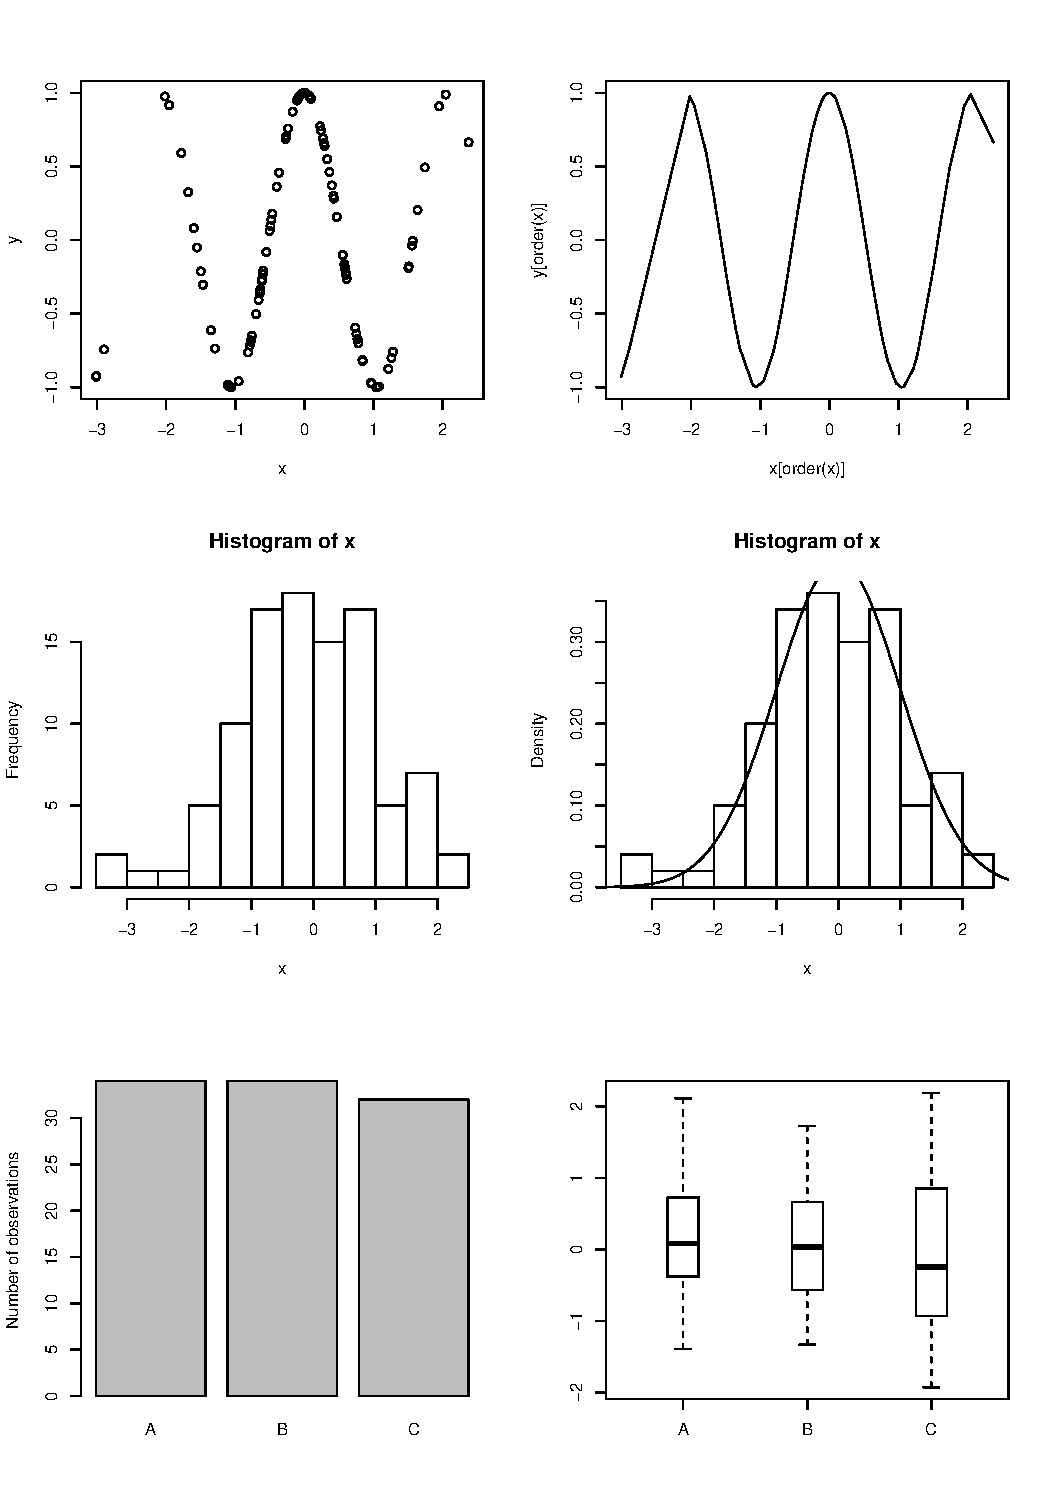
\includegraphics[width=\maxwidth]{figure/unnamed-chunk-16-1} 

\end{knitrout}
\end{figure}

\begin{exercise}
Using the CO2 dataset from exercise \ref{CO2ex}, create a histogram of the variable uptake. Use the information from the help page, \texttt{?hist}, to change the main title and the labels for the x and y axes.
\end{exercise}

\begin{exercise}
Using the CO2 dataset, create a boxplot of uptake seperated by the variables Type and Treatment.
\end{exercise}

\begin{exercise}
Using the CO2 dataset, create a scatterplot with the variable uptake on the y axis and the variable conc on the x axis. Make the observations for Type Quebec a different color from those of Type Mississippi.
\end{exercise}

\section{Functions}
User-defined functions are constructed using the \texttt{function} function (*sigh*). The value of the final line of the function gives the output of the function.
\begin{knitrout}
\definecolor{shadecolor}{rgb}{0.969, 0.969, 0.969}\color{fgcolor}\begin{kframe}
\begin{alltt}
\hlstd{f} \hlkwb{<-} \hlkwa{function}\hlstd{(}\hlkwc{x}\hlstd{)\{}
  \hlstd{y} \hlkwb{<-} \hlstd{x} \hlopt{+} \hlnum{2}
  \hlstd{y}
\hlstd{\}}

\hlkwd{f}\hlstd{(}\hlnum{3}\hlstd{)}
\end{alltt}
\begin{verbatim}
## [1] 5
\end{verbatim}
\begin{alltt}
\hlkwd{f}\hlstd{(}\hlkwd{c}\hlstd{(}\hlnum{3}\hlstd{,} \hlnum{4}\hlstd{))} \hlcom{#The function f acts on both cells in the input vector.}
\end{alltt}
\begin{verbatim}
## [1] 5 6
\end{verbatim}
\end{kframe}
\end{knitrout}
The last call, with a vector as an input, works because the operations in the specific function \texttt{f} work with a vector.
\begin{knitrout}
\definecolor{shadecolor}{rgb}{0.969, 0.969, 0.969}\color{fgcolor}\begin{kframe}
\begin{alltt}
\hlkwd{c}\hlstd{(}\hlnum{3}\hlstd{,} \hlnum{4}\hlstd{)} \hlopt{+} \hlnum{2}
\end{alltt}
\begin{verbatim}
## [1] 5 6
\end{verbatim}
\end{kframe}
\end{knitrout}
Functions can have multiple objects as input and return any object.
\begin{knitrout}
\definecolor{shadecolor}{rgb}{0.969, 0.969, 0.969}\color{fgcolor}\begin{kframe}
\begin{alltt}
\hlstd{g} \hlkwb{<-} \hlkwa{function}\hlstd{(}\hlkwc{x1}\hlstd{,} \hlkwc{x2}\hlstd{)\{}
  \hlstd{y} \hlkwb{<-} \hlkwd{data.frame}\hlstd{(}\hlkwc{var1} \hlstd{=} \hlkwd{c}\hlstd{(}\hlstr{"A"}\hlstd{,} \hlstr{"B"}\hlstd{),}
                  \hlkwc{var2} \hlstd{=} \hlkwd{c}\hlstd{(x1, x2))}
  \hlstd{y}
\hlstd{\}}

\hlkwd{g}\hlstd{(}\hlnum{4}\hlstd{,} \hlnum{6}\hlstd{)}
\end{alltt}
\begin{verbatim}
##   var1 var2
## 1    A    4
## 2    B    6
\end{verbatim}
\end{kframe}
\end{knitrout}

\begin{exercise}
Write a function which takes a vector and returns the second-last element. Note: the \texttt{length} function returns the number of elements in a vector.
\end{exercise}

\begin{exercise}
Given two numerical vectors, $u$ and $v$, of equal length $n$, the squared Euclidean distance is defined by
\begin{equation}
d(v,u)=\sum_{i=1}^n (u_i - v_i)^2.
\end{equation}
For example, the distance between the vectors $v = (1,3,5)$ and $u = (6,3,9)$ is given by
\begin{equation}
\begin{split}
d(v,u) &= (1-6)^2 + (3-3)^2 + (5-9)^2 \\
&= 5^2 + 0^2 + 4^2 \\ 
&= 25 + 0 + 16 \\
&= 41.
\end{split}
\end{equation}
Write a function which takes two equal length vectors as input and returns the squared Euclidean distance.
\end{exercise}

\begin{exercise} \label{halfFun}
A point on the plane can be described as two numbers in a vector of length two $(x,y)$, e.q. $(4,2)$ is the point which is four on the x axis and two on the y axis. Create a function which takes two points in the plane and returns the point which is half-way between the two points. For example, the inputs $(4,2)$ and $(2,8)$ should return $(3,5)$.
\end{exercise}

\section{If-statements}
Operations can be made conditional using an if-statement.
\begin{knitrout}
\definecolor{shadecolor}{rgb}{0.969, 0.969, 0.969}\color{fgcolor}\begin{kframe}
\begin{alltt}
\hlstd{f} \hlkwb{<-} \hlkwa{function}\hlstd{(}\hlkwc{x}\hlstd{)\{}
  \hlkwa{if}\hlstd{(x} \hlopt{>} \hlnum{4}\hlstd{) \{}\hlkwd{print}\hlstd{(}\hlstr{"Greater than four"}\hlstd{)\}} \hlkwa{else}\hlstd{\{}
    \hlkwd{print}\hlstd{(}\hlstr{"Less than or equal to four"}\hlstd{)}
  \hlstd{\}}
\hlstd{\}}

\hlkwd{f}\hlstd{(}\hlnum{3}\hlstd{)}
\end{alltt}
\begin{verbatim}
## [1] "Less than or equal to four"
\end{verbatim}
\begin{alltt}
\hlkwd{f}\hlstd{(}\hlnum{5}\hlstd{)}
\end{alltt}
\begin{verbatim}
## [1] "Greater than four"
\end{verbatim}
\end{kframe}
\end{knitrout}

\begin{exercise}
Create a function which takes a single numerical value as input and returns \texttt{"Even"} if the input is even and \texttt{"Odd"} if the input is odd.
\end{exercise}

\section{For-loops}
For-loops can be used to reproduce a set of code multiple times, cycling through the input.
\begin{knitrout}
\definecolor{shadecolor}{rgb}{0.969, 0.969, 0.969}\color{fgcolor}\begin{kframe}
\begin{alltt}
\hlstd{a} \hlkwb{<-} \hlkwd{c}\hlstd{(}\hlnum{3}\hlstd{,} \hlnum{2}\hlstd{,} \hlnum{5}\hlstd{)}
\hlkwa{for}\hlstd{(i} \hlkwa{in} \hlstd{a)\{}
  \hlkwd{print}\hlstd{(i} \hlopt{+} \hlnum{1}\hlstd{)}
\hlstd{\}}
\end{alltt}
\begin{verbatim}
## [1] 4
## [1] 3
## [1] 6
\end{verbatim}
\end{kframe}
\end{knitrout}
The code in the loop does not have to depend on current value in the loop.
\begin{knitrout}
\definecolor{shadecolor}{rgb}{0.969, 0.969, 0.969}\color{fgcolor}\begin{kframe}
\begin{alltt}
\hlkwa{for}\hlstd{(i} \hlkwa{in} \hlstd{a)\{}
  \hlkwd{print}\hlstd{(}\hlnum{1}\hlstd{)}
\hlstd{\}}
\end{alltt}
\begin{verbatim}
## [1] 1
## [1] 1
## [1] 1
\end{verbatim}
\end{kframe}
\end{knitrout}
For-loops can be used to calculate recursive sequences. Take for example the Fibonacchi sequence defined by
%\begin{equation}
\begin{align*}
& a_0 = a_1 = 1 \\
& a_i = a_{i-1} + a_{i-2} \qquad i \geq 2,
\end{align*}
%\end{equation}
and beginning $(1,1,2,3,5,8,13,21,34,...)$.
\begin{knitrout}
\definecolor{shadecolor}{rgb}{0.969, 0.969, 0.969}\color{fgcolor}\begin{kframe}
\begin{alltt}
\hlstd{n} \hlkwb{<-} \hlnum{10} \hlcom{#The length of the sequence}
\hlstd{a} \hlkwb{<-} \hlkwd{numeric}\hlstd{()} \hlcom{#Sets up an empty numerical vector}
\hlstd{a[}\hlnum{1}\hlstd{]} \hlkwb{<-} \hlstd{a[}\hlnum{2}\hlstd{]} \hlkwb{<-} \hlnum{1} \hlcom{#First two cells are 1}
\hlkwa{for}\hlstd{(i} \hlkwa{in} \hlnum{3}\hlopt{:}\hlstd{n)\{}
  \hlstd{a[i]} \hlkwb{<-} \hlstd{a[i}\hlopt{-}\hlnum{1}\hlstd{]} \hlopt{+} \hlstd{a[i}\hlopt{-}\hlnum{2}\hlstd{]} \hlcom{#Next cell is sum of preceeding two}
\hlstd{\}}

\hlstd{a}
\end{alltt}
\begin{verbatim}
##  [1]  1  1  2  3  5  8 13 21 34 55
\end{verbatim}
\end{kframe}
\end{knitrout}

\begin{exercise}
Create a for-loop which loops over the letters of the alphabet (available as \texttt{LETTERS}) and for each step of the loop adds the new letter to the preceeding letters (so that, for example, the third step is \texttt{"ABC"}) and prints the string of letters. Hint: \texttt{paste} can be used to concatenate two character strings.
\end{exercise}

\begin{exercise}
Create a function which takes a natural number $n$ as input and returns the $n$th Fibonacchi number. 
\end{exercise}

\begin{exercise}
Find the smallest Fibonacchi number greater than $1 000 000$.
\end{exercise}

\begin{exercise}
What happens to the ratio between two Fibonacchi number, $a_i/a_{i-1}$, as $i$ gets larger? Does it converge to some specific number? If so, what is the square of the atomic number of the element associated with that number?
\end{exercise}

\section{Pseudo-random Number Generation} \label{PRNG}
Pseudo-random numbers are numbers created using a deterministic process, intended to emulate completely random numbers. R includes functions to draw numbers from a large number of different distributions.
\begin{knitrout}
\definecolor{shadecolor}{rgb}{0.969, 0.969, 0.969}\color{fgcolor}\begin{kframe}
\begin{alltt}
\hlkwd{par}\hlstd{(}\hlkwc{mfrow} \hlstd{=} \hlkwd{c}\hlstd{(}\hlnum{2}\hlstd{,}\hlnum{2}\hlstd{))}

\hlcom{#Uniform distribution, a = 0, b = 1}
\hlstd{x} \hlkwb{<-} \hlkwd{runif}\hlstd{(}\hlnum{1000}\hlstd{)}
\hlkwd{hist}\hlstd{(x,} \hlkwc{main} \hlstd{=} \hlstr{"U(0,1)"}\hlstd{)}

\hlcom{#Normal distribution, mean = 0, sd = 1}
\hlstd{x} \hlkwb{<-} \hlkwd{rnorm}\hlstd{(}\hlnum{1000}\hlstd{)}
\hlkwd{hist}\hlstd{(x,} \hlkwc{main} \hlstd{=} \hlstr{"N(0,1)"}\hlstd{)}

\hlcom{#Poisson distribution, lambda = 3}
\hlstd{x} \hlkwb{<-} \hlkwd{rpois}\hlstd{(}\hlnum{1000}\hlstd{,} \hlkwc{lambda} \hlstd{=} \hlnum{3}\hlstd{)}
\hlkwd{barplot}\hlstd{(}\hlkwd{table}\hlstd{(x),} \hlkwc{main} \hlstd{=} \hlstr{"Po(3)"}\hlstd{)}

\hlcom{#Binomial distribution, n = 5, p = 0.3}
\hlstd{x} \hlkwb{<-} \hlkwd{rbinom}\hlstd{(}\hlnum{1000}\hlstd{,} \hlkwc{size} \hlstd{=} \hlnum{5}\hlstd{,} \hlkwc{prob} \hlstd{=} \hlnum{0.3}\hlstd{)}
\hlkwd{barplot}\hlstd{(}\hlkwd{table}\hlstd{(x),} \hlkwc{main} \hlstd{=} \hlstr{"Bin(5, 0.3)"}\hlstd{)}
\end{alltt}
\end{kframe}
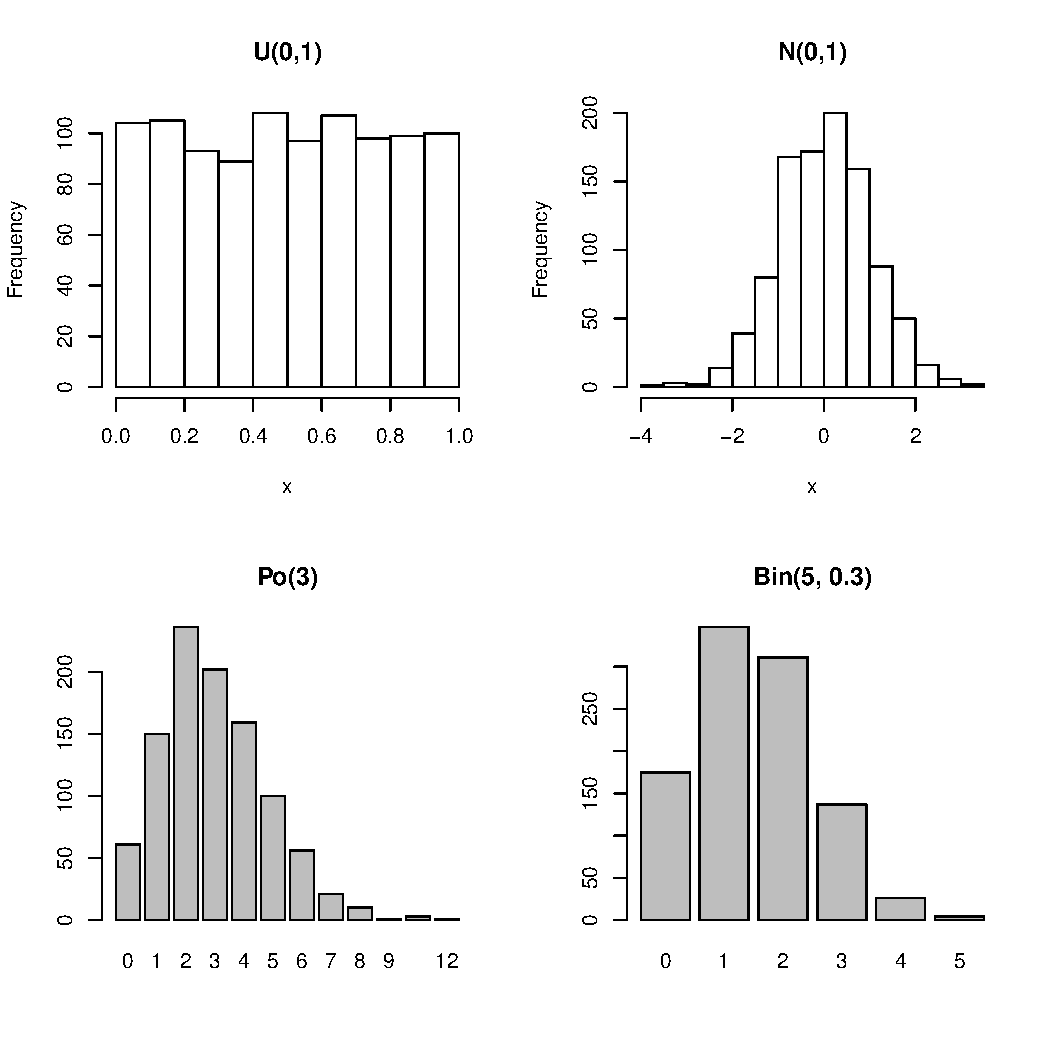
\includegraphics[width=\maxwidth]{figure/unnamed-chunk-24-1} 

\end{knitrout}
Random numbers can be used to test if methods and functions work as intended.
As an example, we investigate the distribution of a mean value. Based on theory, one expects the mean value of $100$ observations from a standard normal distribution to be normal with mean $\mu=0$ and standard deviation $\sigma = 0.1$. To test this, we simulate the situation multiple times and store the mean values.
\begin{knitrout}
\definecolor{shadecolor}{rgb}{0.969, 0.969, 0.969}\color{fgcolor}\begin{kframe}
\begin{alltt}
\hlstd{meanValues} \hlkwb{<-} \hlkwd{numeric}\hlstd{()}
\hlkwa{for}\hlstd{(i} \hlkwa{in} \hlnum{1}\hlopt{:}\hlnum{10000}\hlstd{)\{}
  \hlstd{x} \hlkwb{<-} \hlkwd{rnorm}\hlstd{(}\hlnum{100}\hlstd{,} \hlkwc{mean} \hlstd{=} \hlnum{0}\hlstd{,} \hlkwc{sd} \hlstd{=} \hlnum{1}\hlstd{)}
  \hlstd{meanValues[i]} \hlkwb{<-} \hlkwd{mean}\hlstd{(x)}
\hlstd{\}}

\hlkwd{mean}\hlstd{(meanValues)}
\end{alltt}
\begin{verbatim}
## [1] -0.0007930347
\end{verbatim}
\begin{alltt}
\hlkwd{sd}\hlstd{(meanValues)}
\end{alltt}
\begin{verbatim}
## [1] 0.09975179
\end{verbatim}
\begin{alltt}
\hlkwd{par}\hlstd{(}\hlkwc{mfrow} \hlstd{=} \hlkwd{c}\hlstd{(}\hlnum{1}\hlstd{,}\hlnum{1}\hlstd{))}
\hlkwd{hist}\hlstd{(meanValues,} \hlkwc{prob} \hlstd{= T)}
\hlkwd{lines}\hlstd{(}\hlkwd{seq}\hlstd{(}\hlopt{-}\hlnum{1}\hlstd{,} \hlnum{1}\hlstd{,} \hlnum{0.01}\hlstd{),} \hlkwd{dnorm}\hlstd{(}\hlkwd{seq}\hlstd{(}\hlopt{-}\hlnum{1}\hlstd{,} \hlnum{1}\hlstd{,} \hlnum{0.01}\hlstd{),}
                              \hlkwc{mean} \hlstd{=} \hlnum{0}\hlstd{,} \hlkwc{sd} \hlstd{=} \hlnum{0.1}\hlstd{))}
\end{alltt}
\end{kframe}

{\centering 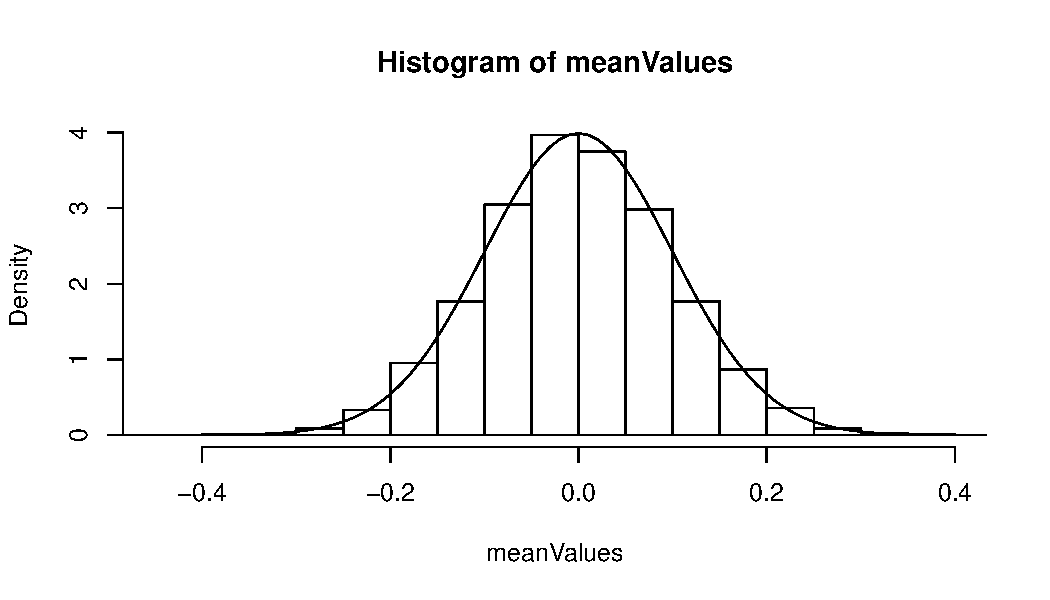
\includegraphics[width=\maxwidth]{figure/unnamed-chunk-25-1} 

}



\end{knitrout}
The simulated result supports the theoretical calculation.

Another common use of random numbers is to evaluate integrals. Recall the intuitive understanding of an integral as an area under a curve. If the curve is contained in a rectangle, and random points simulated in the rectangle, the area under the curve can be estimated as the proportion of points that are below the curve times the area of the rectangle.

For example, take
\begin{equation}
f(x) = \sqrt{1-x^2} \qquad x \in (0,1),
\end{equation}
the curve which gives the upper right part of the unit circle.
\begin{knitrout}
\definecolor{shadecolor}{rgb}{0.969, 0.969, 0.969}\color{fgcolor}\begin{kframe}
\begin{alltt}
\hlstd{x} \hlkwb{<-} \hlkwd{seq}\hlstd{(}\hlnum{0.01}\hlstd{,} \hlnum{0.99}\hlstd{,} \hlnum{0.01}\hlstd{)}
\hlkwd{plot}\hlstd{(x,} \hlkwd{sqrt}\hlstd{(}\hlnum{1} \hlopt{-} \hlstd{x}\hlopt{^}\hlnum{2}\hlstd{),} \hlkwc{type} \hlstd{=} \hlstr{"l"}\hlstd{,} \hlkwc{cex.axis} \hlstd{=} \hlnum{0.5}\hlstd{,}
     \hlkwc{cex.lab} \hlstd{=} \hlnum{0.75}\hlstd{,} \hlkwc{ylab} \hlstd{=} \hlkwd{expression}\hlstd{(}\hlkwd{sqrt}\hlstd{(}\hlstr{"1-x"}\hlopt{^}\hlnum{2}\hlstd{)))}
\end{alltt}
\end{kframe}

{\centering 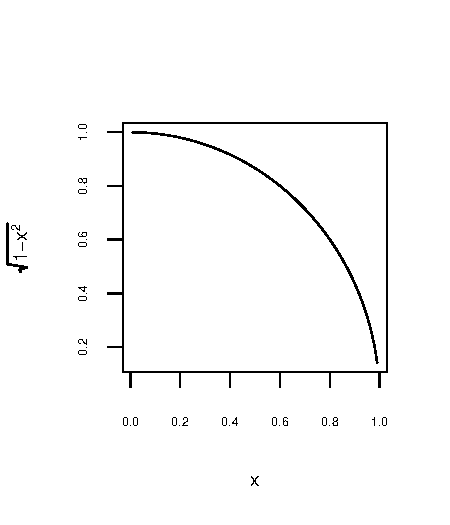
\includegraphics[width=\maxwidth]{figure/unnamed-chunk-26-1} 

}



\end{knitrout}
We simulate from the $1 \times 1$ rectangle with base $(0,0)$ and check if the random number $y$ if smaller than $\sqrt{1-x^2}$ for the random number $x$. The area of the rectangle is $1$, so the estimate of the integral is given directly by the proportion of points below the curve.
\begin{knitrout}
\definecolor{shadecolor}{rgb}{0.969, 0.969, 0.969}\color{fgcolor}\begin{kframe}
\begin{alltt}
\hlstd{underTheCurve} \hlkwb{<-} \hlkwd{numeric}\hlstd{()}
\hlkwa{for}\hlstd{(i} \hlkwa{in} \hlnum{1}\hlopt{:}\hlnum{10000}\hlstd{)\{}
  \hlstd{x} \hlkwb{<-} \hlkwd{runif}\hlstd{(}\hlnum{1}\hlstd{)}
  \hlstd{y} \hlkwb{<-} \hlkwd{runif}\hlstd{(}\hlnum{1}\hlstd{)}
  \hlstd{yUnderCurve} \hlkwb{<-} \hlstd{y} \hlopt{<} \hlkwd{sqrt}\hlstd{(}\hlnum{1} \hlopt{-} \hlstd{x}\hlopt{^}\hlnum{2}\hlstd{)}
  \hlstd{underTheCurve[i]} \hlkwb{<-} \hlstd{yUnderCurve}
\hlstd{\}}
\hlstd{integralEstimate} \hlkwb{<-} \hlkwd{mean}\hlstd{(underTheCurve)}
\hlstd{integralEstimate}
\end{alltt}
\begin{verbatim}
## [1] 0.7936
\end{verbatim}
\end{kframe}
\end{knitrout}
Note that the mean of a logical vector returns the proportion of cells with value \texttt{TRUE}.

Since our integral is one fourth of the unit circle, and the unit circle should have an area given by $\pi$, four times our integral estimate gives an estimate of the constant $\pi \approx 3.14$.
\begin{knitrout}
\definecolor{shadecolor}{rgb}{0.969, 0.969, 0.969}\color{fgcolor}\begin{kframe}
\begin{alltt}
\hlnum{4} \hlopt{*} \hlstd{integralEstimate}
\end{alltt}
\begin{verbatim}
## [1] 3.1744
\end{verbatim}
\begin{alltt}
\hlstd{pi}
\end{alltt}
\begin{verbatim}
## [1] 3.141593
\end{verbatim}
\end{kframe}
\end{knitrout}

\begin{exercise}
Simulate $10$ numbers from a normal distribution with mean $0$ and standard deviation $1$. What is the maximum value? Repeat with $100$ numbers, $1000$ numbers, and so on, until you are bored.
\end{exercise}

\begin{exercise}
Use the simulation approach to evaluate the area under the curve $\sqrt{x+1}$ for $x$ in the interval $(0,2)$, i.e. $x$ between $0$ and $2$. The solution should be close to $2.80$.
\end{exercise}

\begin{exercise}
Use the simulation approach to evaluate the area under the curve 
\begin{equation}
f(x) = \frac{1}{\sqrt{2 \pi}} e^{-\frac{1}{2} x^2}
\end{equation}
for $x$ in the interval $(-1.96,1.96)$. Note that the curve is the density function of a standard normal distribution - what is the probability of being between $-1.96$ and $1.96$?
\end{exercise}

\begin{exercise}
Draw $1000$ numbers from a Poisson distribution with $\lambda = 3$ and $1000$ numbers from a binomial distribution with $n=100$ and $p = 0.03$. Plot the random draws using two bar charts. Are the plots similar?
\end{exercise}

\begin{exercise}
Theory states that a binomial distribution with some $n$ and a probability of $3/n$ approaches a Poisson distribution with $\lambda=3$ as $n$ increases. Examine if this is true by simulating $1000$ random numbers from a binomial with $n$ equal to $10$, $100$, $1000$ and $10000$ and comparing to a distribution of random numbers from the Poisson distribution.
\end{exercise}

\begin{exercise}
Create a vector of points in the two-dimensional plane using the following scheme. 
\begin{enumerate}
\item Let $a=(0,0)$, $b=(1,1)$ and $c=(2,0)$.
\item Let $d_0 = (1,0.5)$.
\item Given $d_{i-1}$, calculate $d_i$ as the point half-way between $d_{i-1}$ and a random choice of $a$, $b$ and $c$.
\item Repeat the previous step until you reach $d_{1000}$.
\item Plot the set of points.
\end{enumerate}
Hint: in exercise \ref{halfFun} you were asked to write a function which takes two points in the plane and returns the point between the two points.
\end{exercise}

\end{document}
